
\chapter{Graph}

\section{Definition Graph}


-Für Dijkstra auf gerichtete Graphen ausgelegt.

Ein \textbf{Graph} G besteht aus einer Menge X [deren Elemente Knotenpunkte genannt werden] und einer Menge U, wobei jedem Element u $\in$ U in eindeutiger Weise ein geordnetes oder ungeordnetes Paar von [nicht notwendig verschiedenen] Knotenpunkten, x,y $\in$ X zugeordnet ist.
Ist jedem u $\in$ U ein geordnetes Paar von Knoten zugeordnet, so heißt der Graf \textbf{gerichtet}, und wir schreiben 
	$G= (X, U)$.
Die Elemente von U werden in diesem Fall als \textbf{Bögen} bezeichnet.

Ist jedem u $\in$ U ein ungeordnetes Paar von Knotenpunkten zugeordnet, so heißt der Graph \textbf{ungerichtet} und wir schreiben 
	$G=[X,U]$. 
Die Elemente von U bezeichnen wir dann als \textbf{Kanten.}
 \footnote{\cite{Bieß:9}}


Ein gerichteter Graph besteht somit aus einer Menge aus geordneten Knotenpunkten. Dadurch, das diese Punkte geordnet sind, ist eine Verlaufsrichtung festgelegt, in welcher der Graph zeigt.
Somit kann sich eine geometrische Figur ergeben.


Wenn man diese Punkte als Richtungen nun als Straßennetz sähe, würde sich durch die Punkte ein Straßenverlauf abbilden mit unterschiedlichen Verlaufsrichtungen.
Somit verbünde nicht jede Strecke direkt jeden Punkt. Um jenen kürzesten Weg zu finden, der zwei bestimmte Punkte miteinander verbindet, kann man den Dijkstra-Algorithmus anwenden, welcher im Folgenden erklärt wird.



\section{Datenstrukturen zur Repräsentation von Graphen}

\textbf{Speicherung in einer Adjazenzmatrix} \\
Der Graph G=(V,E) wird in einer booleschen m*m Matrix gespeichert ($m = \sharp V$), mit 1 falls $(i,j) \in E$ und 0 falls nicht. \\
Nachteil: Dies erfordert unverhältnismäßig viel Speicher, wenn der Graph nur wenig    	  Kanten hat. Abhilfe schafft eine Zusatzmatrix, die nur bedeutsame Einträge speichert.
 Insgesamt ist eine Adjazenzmatrix aber trotzdem ineffizient bei Graphen mit wenig Kanten. \\
 

\begin{figure}[h]
\centering
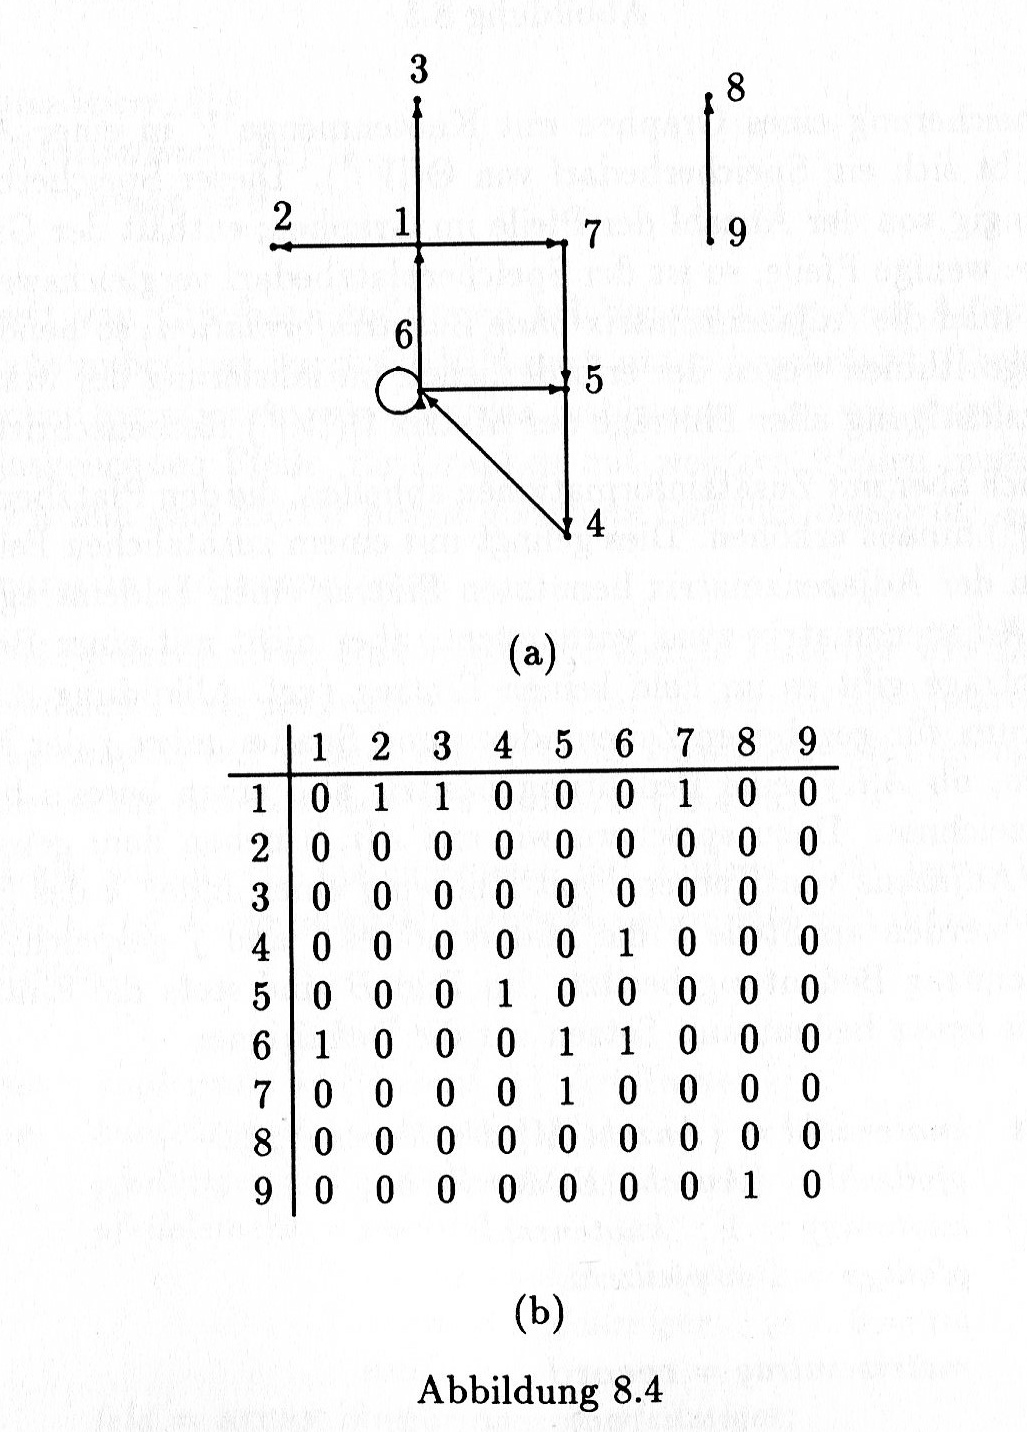
\includegraphics[width = 8cm]{./chapters/adjazenzmatrix.jpg}
\caption{Adjazenzmatrix {\tiny (Quelle: OTTMANN, Thomas; WIDMAYER Peter: Algorithmen und Datenstrukturen, Reihe Informatik Bd. 70, Mannheim: BI-Wissenschaftsverlag, 1990, S.539 Abb. 8.4)} }
\label{a2}
\end{figure}
 
\textbf{Speicherung in Adjazenzlisten}\\
Für jeden Knoten wird eine lineare, verkettete Liste seiner ausgehenden Kanten gespeichert.
Die Knoten werden als lineares Feld gespeichert (d.h. jeder Knoten im Feld zeigt auf eine Liste). \\
Dies ist effizienter als eine Adjazenzmatrix, weil kein Speicherplatz verschwendet wird. \\

\begin{figure}[h]
\centering
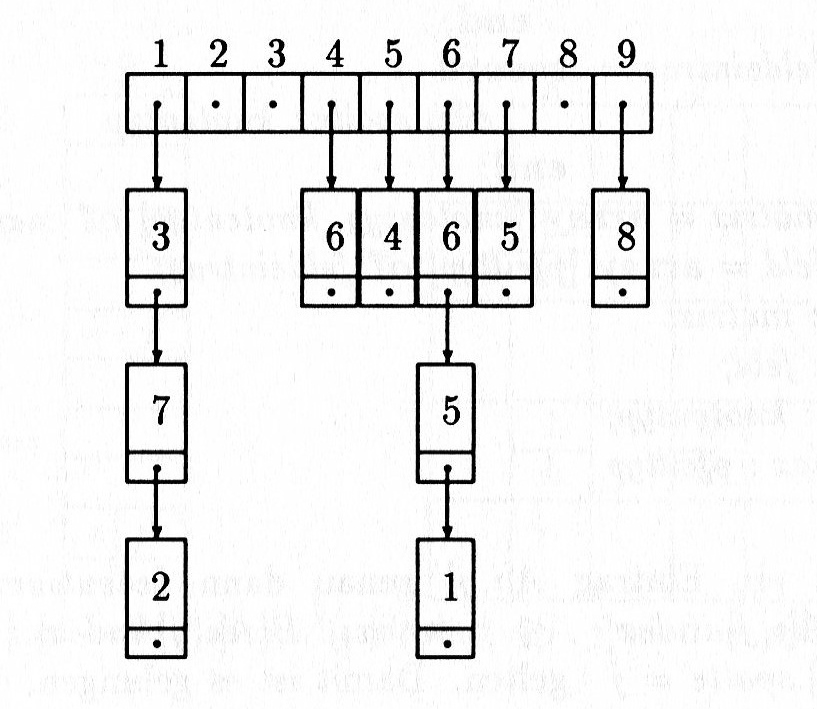
\includegraphics[width = 8cm]{./chapters/adjazenzliste.jpg}
\caption{Adjazenzliste {\tiny (Quelle: OTTMANN, Thomas; WIDMAYER Peter: Algorithmen und Datenstrukturen, Reihe Informatik Bd. 70, Mannheim: BI-Wissenschaftsverlag, 1990, S.542 Abb. 8.6)} }
\label{a3}
\end{figure} 

\textbf{Speicherung in doppelt verketteten Listen}\\
Jedes Element enthält Zeiger auf die beiden Nachbarelemente sowie auf eine Kantenliste (wie bei Adjazenzliste, s.o.).
Diese Darstellung besitzt die den Adjazenzlisten fehlende Dynamik, ist aber natürlich komplizierter.

\begin{figure}[h]
\centering
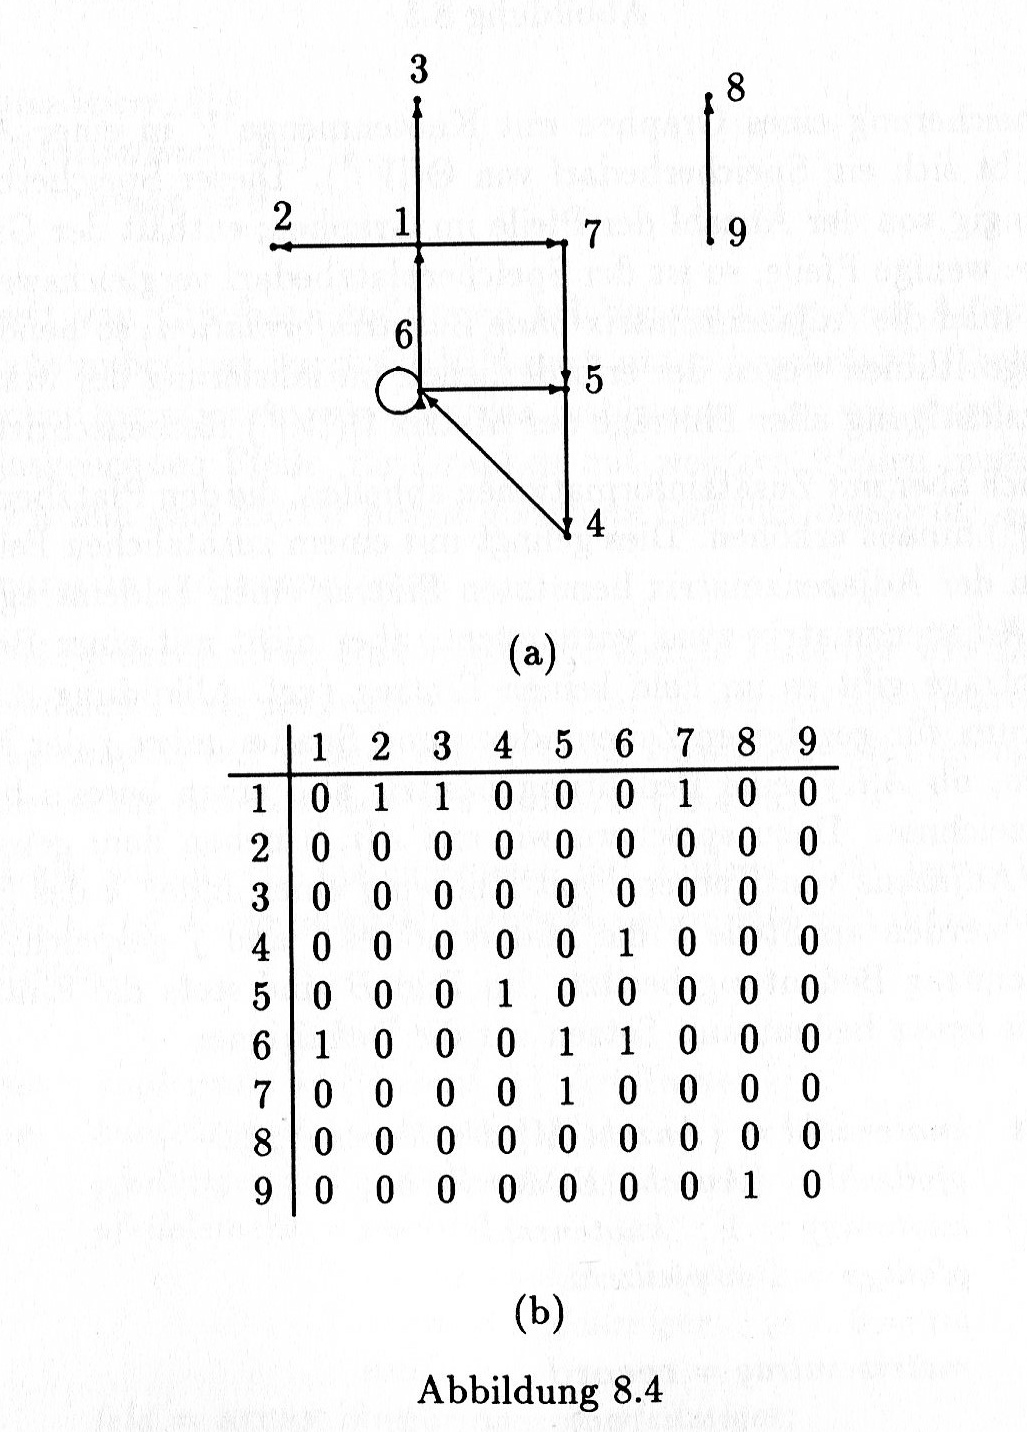
\includegraphics[width = 8cm]{./chapters/adjazenzmatrix.jpg}
\caption{doppeltVerkettetePfeilliste.jpg {\tiny (Quelle: OTTMANN, Thomas; WIDMAYER Peter: Algorithmen und Datenstrukturen, Reihe Informatik Bd. 70, Mannheim: BI-Wissenschaftsverlag, 1990, S.543 Abb. 8.7)} }
\label{a4}
\end{figure}

Quelle:
Algorithmen und Datenstrukturen, T.Ottmann/P.Widmayer, Kap. 8 Graphenalgorithmen, S.539-544
